%!TEX root = practicum1.tex
\subsection*{Convex Hull}
	To find the convex hull of the generated set we use the ConvexHull algorithm given in the exercise. Since the code necessary to compute \t{L\_upper} and \t{L\_lower} is comparative it has been extracted to a method called \t{half\_convex\_hull} provided in \autoref{lst:c:halfConvexHull}. The function \t{half\_convex\_hull} uses the method \t{make_right)turn} that determines if the path defined by the last three points in the set \t{L} makes a right turn. This method, uses the value of $q$ defined in \eqref{eq:b:q}, see \autoref{lst:c:makeRightTurn}. 

	This method is called twice to compute the convex hull, see \autoref{lst:c:convexHull}.

	\lstinputlisting[float, firstline=48, lastline=64, label={lst:c:halfConvexHull}, caption={Method that computes the upper (or lower) half of the convex hull.}]{../assignment1C.py}

	\lstinputlisting[float, firstline=42, lastline=45, label={lst:c:makeRightTurn}, caption={Method that computes the type of a path defined by \t{p1}, \t{p2} and \t{p3}.}]{../assignment1C.py}

	\lstinputlisting[float, firstline=66, lastline=73, label={lst:c:convexHull}, caption={Method that computes the convex hull of the inputted set of points.}]{../assignment1C.py}

	See \autoref{subfig:c:convexHull} for a visualization of a convex hull of 1000 points, generated with the provided \t{generate\_points()} method. \autoref{subfig:c:convexHullTest} shows the convex hull of 100 points and all possible straight lines between points in the set in green, showing that the convex hull is indeed convex.

	\begin{figure}
		\centering
		\begin{subfigure}[t]{0.45\textwidth}
			\centering
			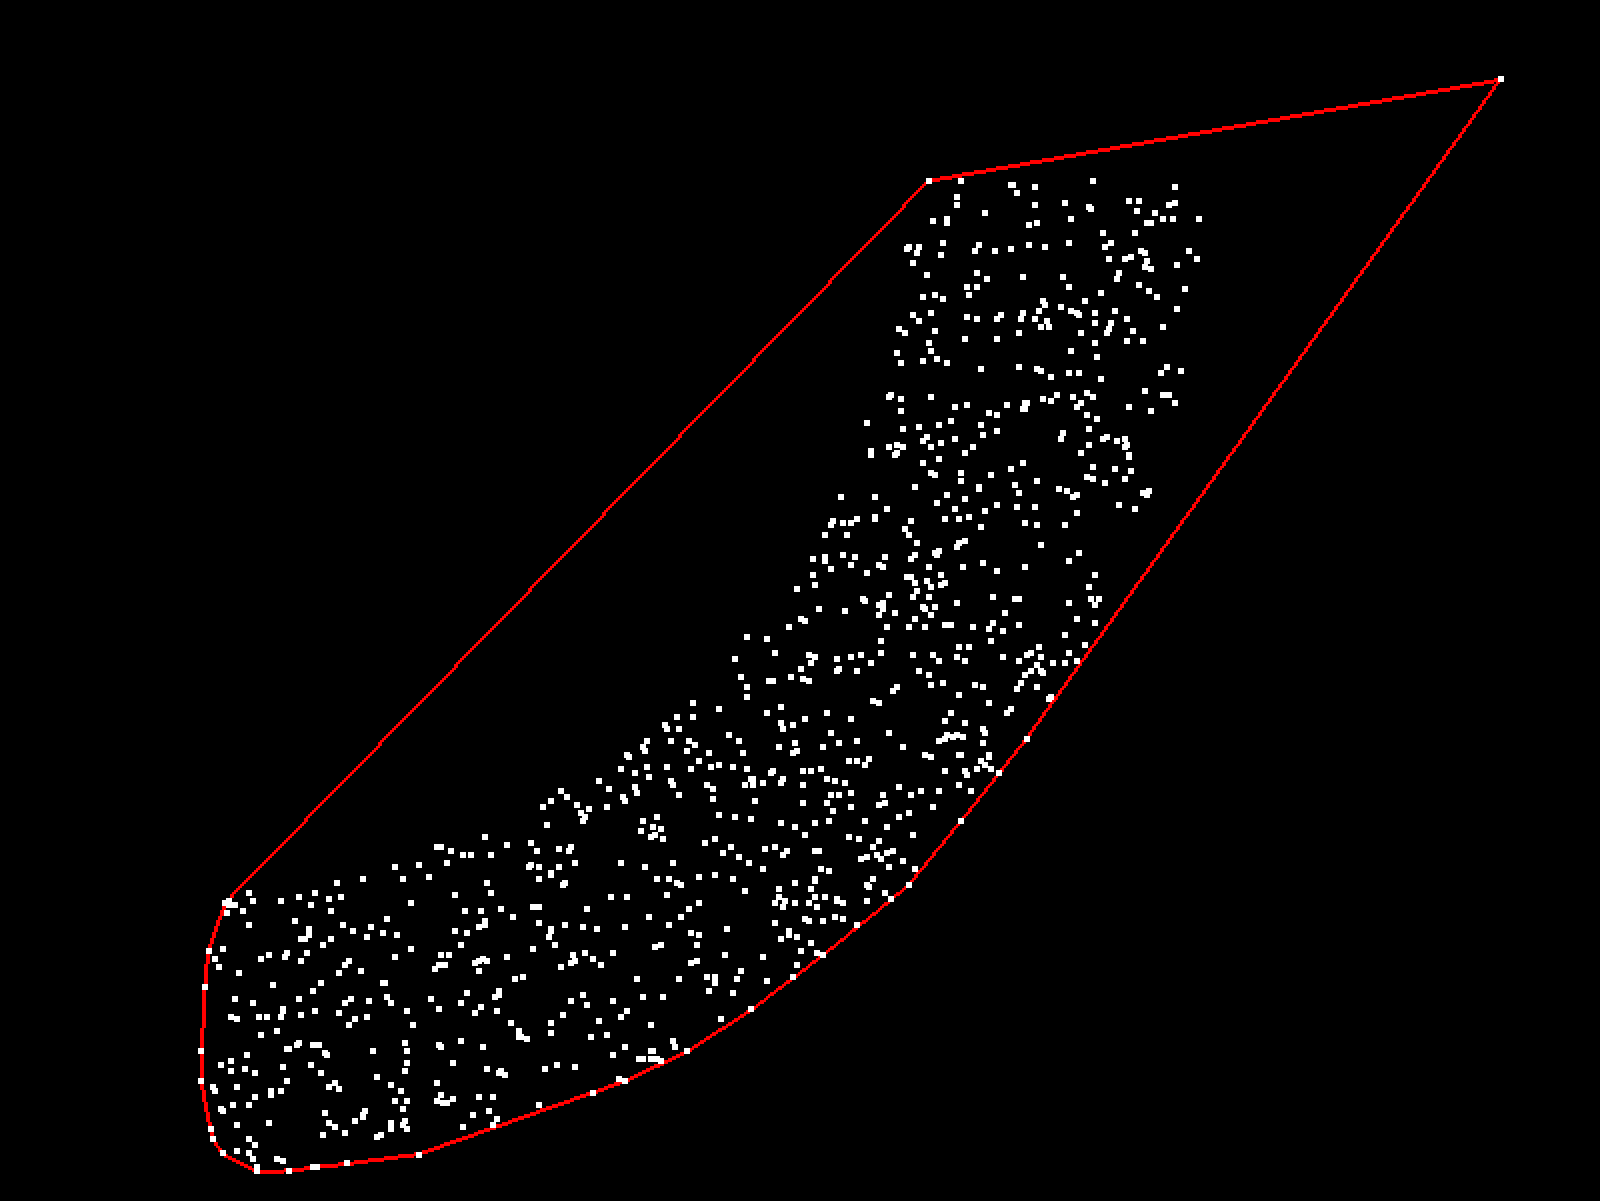
\includegraphics[width=\textwidth]{./img/c_convexHull}
			\caption{Convex hull of 1000 points.}
			\label{subfig:c:convexHull}
		\end{subfigure}
		\begin{subfigure}[t]{0.45\textwidth}
			\centering
			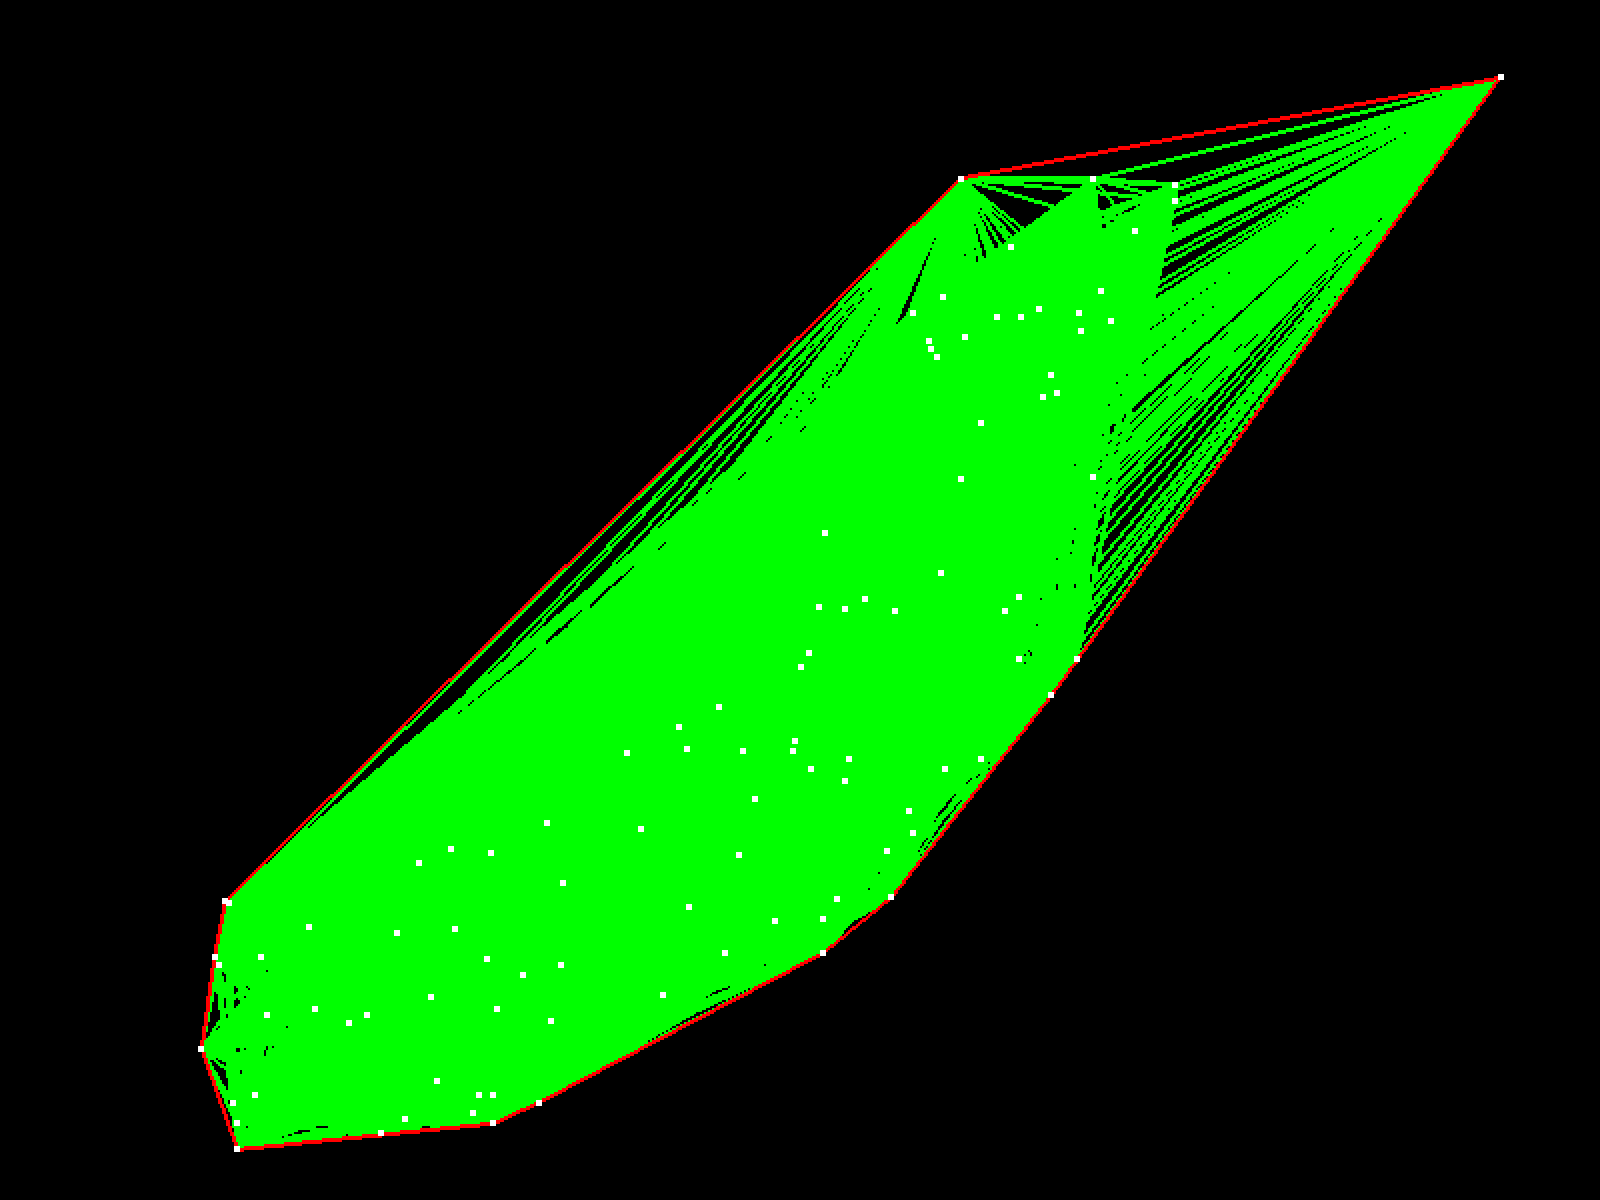
\includegraphics[width=\textwidth]{./img/c_convexHullTest}
			\caption{Convex hull of 100.}
			\label{subfig:c:convexHullTest}
		\end{subfigure}	
		\caption{Visualizations of the convex hull, shown in red, of a set of points, with in (\subref{subfig:c:convexHullTest}) not only the convex hull but also all possible straight lines between points in the set, shown in green.}
		\label{fig:c:convexHulls}
	\end{figure}

\subsection*{Area}
The area $A$ of a irregular planar non-intersecting polygon with vertices $(x_1, y_1),$ $\ldots, (x_n, y_n)$ is defined as:
	\begin{equation}\label{e:barwq}
		\begin{split}
		A 	&= \frac{1}{2} \cdot
				\begin{vmatrix}x_1 & x_2\\y_1 & y_2\end{vmatrix} +
				\begin{vmatrix}x_2 & x_3\\y_2 & y_3\end{vmatrix} +
				\ldots +
				\begin{vmatrix}x_n & x_1\\y_n & y_1\end{vmatrix}\\		
		~	&=					\frac{1}{2} \cdot(
							x_1 \cdot y_2 - 
							x_2 \cdot y_1 + 
							x_2 \cdot y_3 -
							x_3 \cdot y_2\\
			&	\quad\quad\quad		+ \ldots + \\
			&	\quad\quad\quad		x_{n-1} \cdot y_n -
							x_n \cdot y_{n-1} +
							x_n \cdot y_1 -
							x_1 \cdot y_n).
		\end{split}
	\end{equation}
Using this formula, the method to compute the area of a irregular polygon is implemented as in \autoref{lst:c:polygonArea}.

\lstinputlisting[float, firstline=30, lastline=39, label={lst:c:polygonArea}, caption={Method that computes the area of an irregular polygon.}]{../assignment1C.py}